A traffic circle is a type of circular intersection.  It contains a center island, around which traffic flows in one direction.  A traffic circle can have one or multiple lanes inside of it, concentric about its center island.  Also referred to as a rotary or roundabout, it is capable of handling multiple street inputs.  They are commonly utilized throughout New England and Europe.

\begin{figure}[!htbp]
\centering
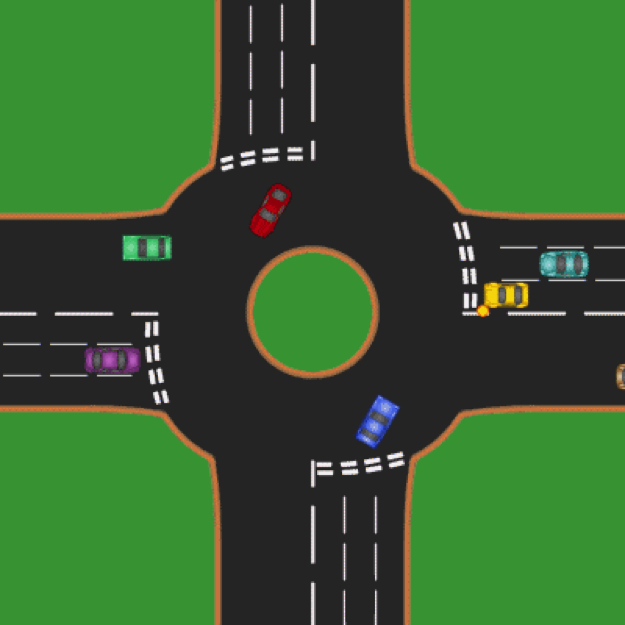
\includegraphics[width=0.5\textwidth]{roundabout}
\caption{A typical traffic circle for a four way intersection\cite{rabout1}}\label{fig:roundabout}
\end{figure}

Unlike a traditional intersection between two perpendicular streets, traffic circles generally do not have traffic lights controlling the flow of traffic.  Rather, traffic is controlled by right of way rules.  Typically, cars already in the traffic circle have right of way over cars seeking to enter into the traffic circle \cite{rabout2}.  Thus, they are designed to slow traffic.  Entering traffic typically yields to traffic already in the rotary, and allows for continuous flow of traffic to multiple exits.

Roads can enter a traffic circle radially or tangentially. Roads that enter radially require slowing down of speed and making a turn, thus acting as a traffic calming measure.  Roads that enter tangentially do not require as much reduction in speed or turn angle, so traffic is not slowed down as much \cite{rabout3}.  Though not as common, entry into traffic circles can also be regulated by traffic lights or stop signs.  

Another advantage of roundabouts is that they allow for easy exit to any of the roadways that connect to it.  With a normal perpendicular intersection, vehicles wanting to make left or right hand turns instead of continuing straight must wait for specific light signals to turn onto the desire road.  With a roundabout, a vehicle simply stays in the traffic circle until reaching its desired exit, which even allows for legal u-turns \cite{rabout1}.

\begin{figure}[!htbp]
\centering
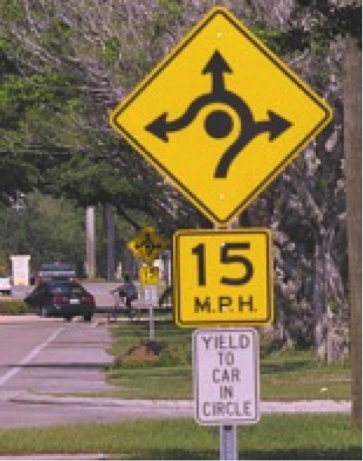
\includegraphics[width=0.5\textwidth]{roundabout-signage}
\caption[Roundabout Signage]{Entering traffic must slow and yield to vehicles already in the circle}\label{fig:roundabout-signage}
\end{figure}

\subsubsection{Advantages and Disadvantages}
The advantages of roundabouts are:\begin{itemize}
	\item Eliminates T-bone (perpendicular) crashes and head on collisions
	\item Allows for continuous entering and exiting of traffic to any street
	\item Improved flow over traffic lights
	\item Calms traffic by reducing speed without complete stops
\end{itemize}

Roundabouts come with the following drawbacks:\begin{itemize}
	\item Lacks computerized traffic control features
	\item Can become congested
	\item Not efficient at moving high volumes of vehicles
	\item Confusing for inexperienced drivers
	\item Require driver decision making and timing
\end{itemize}

\subsubsection{Capacity}
The capacity of a roundabout is dependent upon the number of lanes within the circle, as well as the diameter of the circle.  Most modern roundabouts are less than 250 feet in diameter \cite{rabout1}.  Since it does not necessarily require a full stop by entering vehicles, traffic circles can provide less delay than light controlled intersections.  When the volume of entering traffic is unequal between the different roads (unbalanced), there can be inefficiencies.  Traffic lights are optimized to maximize the traffic throughput by giving more green lights to a busier road, whereas with a roundabout all roads must slow down and yield to traffic within the roundabout, regardless of the amount of traffic on any particular road \cite{rabout4}.  On the other hand, when all of the entering roads experience constant and balanced traffic, a traffic circle can reduce wait times by eliminating red lights.  

\begin{figure}[!htbp]
\centering
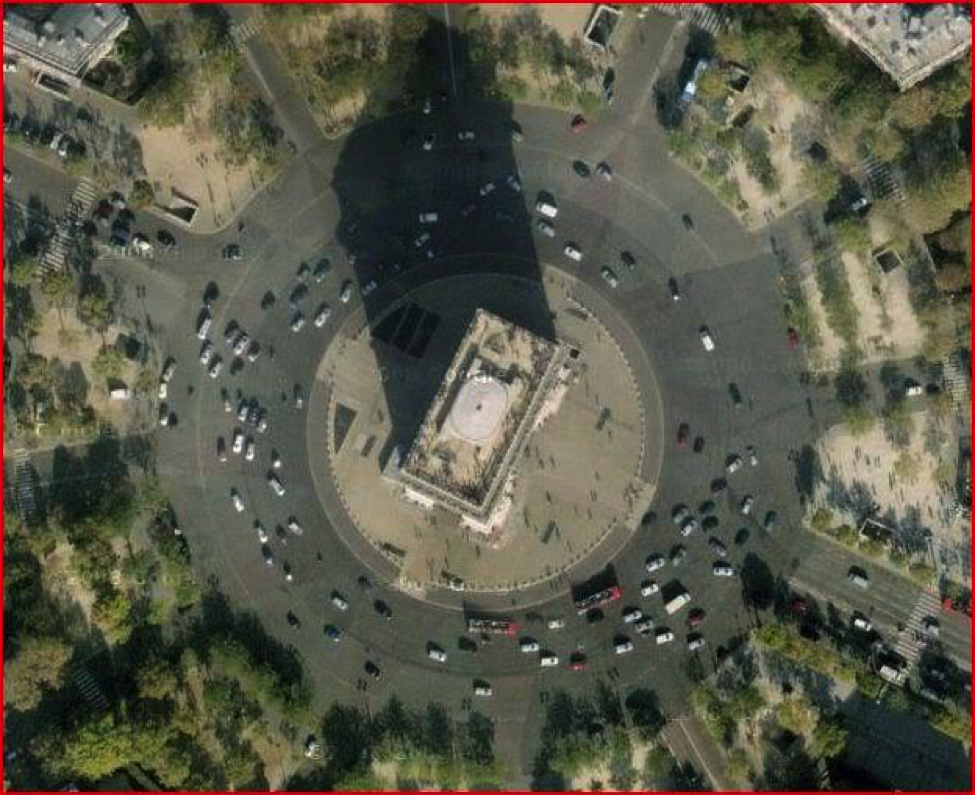
\includegraphics[width=0.5\textwidth]{arc-de}
\caption[Place de l’Etoile]{Perhaps the most well-known traffic circle is the Place de l’Etoile around the Arc de Triomphe in Paris, which has eight lanes with twelve avenues feeding into it.}\label{fig:arc-de}
\end{figure}

\clearpage

\subsubsection{Mini-roundabouts}
One specific type of traffic circle is a mini-roundabout.  Mini-roundabouts can be built in places where there is not enough space for a traditional roundabout.  They are used in place of a four way stop or traffic light controlled intersection.  They improve efficiency by eliminating the delay caused by stop signs and traffic signals.

\begin{figure}[!htbp]
\centering
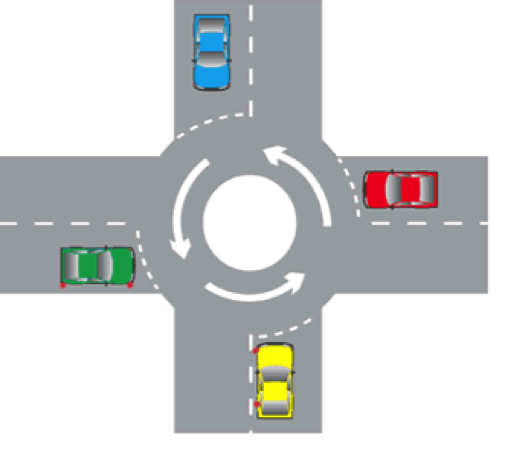
\includegraphics[width=0.5\textwidth]{mini-rabout}
\caption[Mini-Roundabout]{Mini-roundabouts offer greater efficiency than stop signs or lights for intersections with single lane roads.}\label{fig:mini-rabout}
\end{figure}
